\documentclass[a4paper,12pt,openright,twoside,table,xcdraw]{mwbkfixed}
\usepackage[utf8]{inputenc}
\usepackage[OT4]{fontenc}
\usepackage[MeX]{polski}
\usepackage[polish]{babel}
\usepackage[style=ieee, citestyle=numeric-comp,backend=biber,sorting=nyt, defernumbers=true]{biblatex}
\usepackage{caption}
\usepackage{subcaption}
\usepackage{amsmath}
\usepackage{amsfonts}
\usepackage{numprint}
\usepackage{rotating}

\usepackage{blindtext}
\usepackage{bookmark}
\usepackage{hyperref}
\usepackage{ntheorem}
\usepackage{hyperref}
\usepackage{url}
\usepackage{graphicx}

\usepackage[usenames]{color}
\usepackage{enumerate}
\usepackage{pdfpages} 
\usepackage[notintoc, polish]{nomencl}
\usepackage{listings}
\usepackage{lscape} %do tekstu obróconego o~90 stopni
\usepackage{stmaryrd} %niektóre symbole matematyczne
\usepackage{indentfirst}
\usepackage{multirow}
\usepackage{booktabs}
\usepackage{float}
\usepackage{longtable} %łamanie tabel
\usepackage[toc,page]{appendix}
\usepackage{tikz}
\usepackage{enumitem}
\usepackage{textcomp}
\usepackage{multirow}
\usepackage{graphics}
\usepackage{gensymb}
\usepackage{epstopdf}
\usepackage{mathtools}
\usepackage{float}
\usepackage{sidecap}
\usepackage{textcomp}
\usepackage{pgfplots}
\usepackage{epstopdf}
\usepackage{listings}
\usepackage{array}
\usepackage{tabularx}
\usepackage{cases}
\usepackage{indentfirst}
\usepackage{MnSymbol}%
\usepackage{wasysym}%
\usepackage{footnote}


\addbibresource{main.bib}
\npdecimalsign{.}
\nprounddigits{2}


\DeclareGraphicsExtensions{.eps}
\usetikzlibrary{patterns}
\pgfplotsset{width=12cm,compat=1.14}
\usetikzlibrary{arrows,shapes,positioning,shadows,trees,shapes.geometric}
%%%%%%%%%%%%%%%%%%%%%%%%%%%%%

\definecolor{gray80}{gray}{0.8}
\definecolor{chartreuse(traditional)}{rgb}{0.87, 1.0, 0.0}
\definecolor{sepia}{rgb}{0.44, 0.26, 0.08}
\definecolor{turquoise}{rgb}{0.25 0.87 0.81}
\definecolor{mulberry}{rgb}{0.77 0.29 0.55}

\definecolor{codegreen}{rgb}{0,0.6,0}
\definecolor{codegray}{rgb}{0.5,0.5,0.5}
\definecolor{codepurple}{rgb}{0.58,0,0.82}
\definecolor{backcolour}{rgb}{0.95,0.95,0.92}

\begin{document}

\begin{savenotes}
	\begin{figure}[!htb]
		\centering
		\begin{minipage}{.18\textwidth}
			\centering
			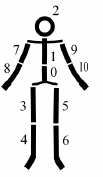
\includegraphics{images/hierarchical-structure.png}       
		\end{minipage}%
		\hfill
		\begin{minipage}{0.75\textwidth}
			\centering
			\scalebox{0.73}{
				\tiny
\begin{tikzpicture}[
	level 1/.style={sibling distance=5.3cm},
level 2/.style={sibling distance=2.3cm}, 
	every node/.style = {shape=rectangle, rounded corners,
    draw, align=center}]]
  \node {0. Miednica\\(\emph{ang. Pelvis})\\6 DOF}   
    child { node {3. Lewe udo\\(\emph{ang. Upper Right Leg})\\2 DOF}
    	child { node {4. Lewy piszczel\\(\emph{ang. Right Lower Leg})\\1 DOF}}
    }
    child { node {1. Kręgosłup\\(\emph{ang. Spine})\\3 DOF}    	
    	child {node{7. Prawe ramię\\(\emph{ang. Upper Right Arm})\\3 DOF}
    		child {node{8. Prawe przedramię\\(\emph{ang. Right Forearm})\\1 DOF}}
    	}
    	child {node{2. Głowa\\(\emph{ang. Head})\\3 DOF}}
	child {node{9. Lewe ramię\\(\emph{ang. Upper Left Arm})\\3 DOF}
		child {node{10. Lewe przedramię\\(\emph{ang. Left Forearm})\\1 DOF}}
	}	     
    }
    child { node {5. Prawe udo\\(\emph{ang. Upper Left Leg})\\2 DOF}
    	child { node {6. Prawy piszczel\\(\emph{ang. Left Lower Leg})\\1 DOF}}
    };
\end{tikzpicture}
			}
		\end{minipage}
		\caption[Uproszczony hierarchiczny model szkieletowy człowieka wraz z~diagramem przedstawiającym hierarchię poszczególnych elementów]{Uproszczony hierarchiczny model szkieletowy człowieka (lewy) wraz z~diagramem przedstawiającym hierarchię poszczególnych elementów(prawy) \cite{Kwolek2014}}
		\label{fig:literature:skeletonModelHierarchy}
	\end{figure}
\end{savenotes}	

\end{document}